% !TEX root = ../main.tex
\section{Introduction}\label{sec:rfs-introduction}
% !TEX root = ../../main.tex
% \newcommand\x{\scalebox{1.6}{\textbullet}}
\begin{table*}[t]
    \begin{center}
    \resizebox{1.0\textwidth}{!}{%
    \begin{tabular}{@{}lccccccccc|cccccc@{}}
      & \multicolumn{9}{c}{\bf Attributes} & \multicolumn{5}{c}{\bf                                                 Users}\\
      \cmidrule(lr){2-10} \cmidrule(lr){11-15}
      {\bf Items} & Pizza & Eggs & Taco & Salad & Avocado & Chicken & Sardines & Beer & Coffee & 1 & 2 & 3 & 4 & 5 \\
      Morning Pizza & \x & \x & & & & & & & \x & & \x & & \x & \\
      Dinner Pizza & \x & & & & & & \x & \x & & \x & & & \x & \\
      Small Salad & & & & \x & \x & & \x & & & & & \x & & \x \\
      Big Salad & & \x & & \x & \x & \x & & & \x & & & \x & \x & \\
      Taco & & & \x & & \x & \x & & & \x & & & &  & \x \\
      Fish Taco & & & \x & & & & \x & & & & \x &  & \x & \\
      \bottomrule
    \end{tabular}
    }
    \caption[Example recommender systems data of items with attributes]{\label{tab:example-meals}An example of the data we focus on, where tagged items are recommended to users based on both item attributes and items users have consumed in the past. This example dataset of meals contains meals with different foods (left) and users log which meals they ate (right). The goal is to leverage the attributes to recommend items to users.
    }
    \end{center}
\end{table*}
Classical recommender system datasets contain a matrix where each row is a user and each column is an item. Each entry in the matrix indicates whether or not a user consumed an item. Modern applications often gather rich side information about items in the form of a set of attributes or tags. Item attributes provide valuable side information for recommender systems. With a large number of items or a sparse user-item matrix, attribute information is necessary for good performance.

We are motivated by a specific dataset with these properties: a dataset of 55k users logging 16M meals using the LoseIt! diet tracking app. \Cref{tab:example-meals} shows the kind of data logged by users, where each row is an item (meal), each left-hand column is an attribute (food), and each right-hand column is a user. The food attributes can clearly inform recommendations: User~1 does not log meat, User~4 is omnivorous and undiscriminating, and User 3 mostly eats salads. In the LoseIt! data, there is a massive number of possible items to recommend: there are 12M unique meals, composed of subsets of 3M foods. Meals containing only a few foods, or those ordered at chain restaurants, may be logged by many users. But these represent a small proportion of the meals people actually eat, so a long tail of meals are logged by single users.
%Models that require parameters to be learned for every item cannot scale to this type of data, and models that do not leverage attributes cannot recommend items from the long tail.

Modeling item attributes in these non-standard recommender systems is not straightforward. Popular ways to use item attributes like multiple matrix factorization~\citep{wang2011collaborative,gopalan2014content-based} struggle when the attribute vocabulary or number of items is large. Conversely, simple models are computationally tractable but risk losing the ability to capture nonlinear patterns of user consumption. For instance, a user may enjoy meals tagged with foods \texttt{A} and \texttt{B}, \texttt{B} and \texttt{C}, or \texttt{A} and \texttt{C}, but not all three. Finding the right balance between scalability and flexibility is therefore a primary goal.

Even when a model can be scaled, it may not be clear how its training procedure
connects to the recommender system evaluation metric.
% A model optimized using a training objective may not yield optimal recommendation performance.
A matrix factorization method might minimize mean squared error when the recommender
system is evaluated on recall. While it is plausible that minimizing mean squared error will
improve recall, the connection between the two is implicitly assumed in many methods. Ideally, a recommender system should have an objective that matches its evaluation metric.

This paper proposes \gls{rfs}, a class of principled, scalable models for recommending items with sets of attributes. \gls{rfs} casts the recommendation problem as binary classification. Given a user and an item, \gls{rfs} treats attributes as features and classifies whether or not the item is likely to be consumed by the user. \gls{rfs} learns embeddings for each user and attribute; each item is represented as the mean of its attribute embeddings. To scale to large datasets, we develop an \gls{rfs} method that is trained using negative sampling of random items that are unlikely to be consumed.

\gls{rfs} enjoys two benefits from framing the recommendation problem as classification. First, the \gls{rfs} classification objective function is directly tied to recommender recall: we show that a classifier with zero worst-case error achieves maximum recall. Second, \gls{rfs} is provably flexible enough to learn any class of recommendation model based on set-valued side information (including multiple matrix factorization). This generality makes \gls{rfs} a natural drop-in replacement for many specialized models in the literature.

We study the performance of the negative sampling \gls{rfs} model on a semi-synthetic benchmark dataset and the LoseIt! dataset. The semi-synthetic paper recommendation dataset consists of 65k users clicking on 636k papers posted to the arXiv; the attributes of each paper are the unique words in its abstract. We then apply the method to the LoseIt! dataset to make out-of-sample meal recommendations. In both cases, the \gls{rfs} method outperforms the state of the art in terms of recall. In addition to good performance, the \gls{rfs} model learns interpretable embeddings that intuitively capture the structure of the underlying data.
% !TEX root = ../../main.tex
\begin{figure*}[p!]
  \centering
%  \pdfimageresolution=500
  \includegraphics[width=1.0\textwidth]{ch-rfs/fig/arxiv_user_embeddings_tsne.png}
  \caption[Qualitative evaluation of \textsc{rfs} on arXiv reading behavior data]{\label{fig:arxiv_tsne} \textbf{\acrlong{rfs} trained on arXiv reading behavior clusters researchers by their most frequently-read arXiv category (best viewed on a screen).} \gls{rfs} is trained to recommend items using their attributes (words in the abstract). t-SNE~\citep{maaten2008visualizing} is used to visualize the user embeddings $\theta_u$ in the inner product regression function in \Cref{eqn:rankfromsets}. Each marker represents a user embedding; its color represents a user's most-read arXiv category. Unique colors are determined using the most-read categories across the arXiv, and colors are assigned according to the arXiv ontology. \gls{rfs} captures usage patterns, as fields of study are related by patterns of reading behavior across neighboring fields (e.g. \texttt{stat.ML} and \texttt{cs.IT}).} %An interactive map with all labels can be accessed at %\href{http://j.mp/rankfromsets}{\texttt{http://j.mp/rankfromsets}}.}
\end{figure*}
\clearpage

% \gls{rfs} is extremely scalable and is fit with a loss function tied to an
% evaluation metric. In addition to outperforming competitors on large datasets,
% it is backed by an ability to approximate other models that recommend items with
% attributes. \emph{This work demonstrates that if a practitioner aims to perform
%   recommendation of items with attributes and measures recommendation
%   performance with recall, the best choice of model is a deep classifier such as
%   \gls{rfs}.}
% The rest of this paper is organinized as follows:
% \paragraph{Background}
% \begin{itemize}
%     \item Recommendation with side information
%     \item Negative sampling in recommender systems
%     \item Regression models with set-valued features
% \end{itemize}
% \paragraph{Method}
% \begin{itemize}
%     \item Recommendation as classification
%     \item Embedding users and items
%     \item Learning the parameters through negative sampling
% \end{itemize}

% \paragraph{Results}
% \begin{itemize}
%     \item Metrics (recall@K definition)
%     \item Recommending documents
%     \item Recommending meals
% \end{itemize}
% \paragraph{Discussion}
% \begin{itemize}
%     \item Summarize contribution
%     \item Incorporating additional side information
%     \item Other interesting things?
% \end{itemize}
% % set up the task of recommendation, foreshadow how we will solve it via
% % classification
% Sets of attributes represent many types of items. A user might be associated
% with a photo that has tags, a disease with diagnosis codes, or a playlist of
% songs. Recommendation models for such items use the item attributes to rank
% items for users. Central to building recommendation models is evaluation, and a
% common metric is recall. But existing models such as matrix factorization do not
% have associated theoretical guarantees of improved recall. Currently, models are
% built on a case-by-case basis and adapted to the data at hand, and must be
% painstakingly compared to see which extension leads to improvement of the
% evaluation metric.
% % foreshadow desiderata
% Our goal is to build a recommendation model to rank items from attributes, and
% buttress the model with theoretical guarantees of universal approximation
% (ability to approximate other models) and of improved recommendation performance
% vis-\`a-vis recall.
% % desideratum #1: statistical challenge
% Building models that rank items from sets of attributes must address two
% difficulties arising from the properties of sets. The first difficulty is the
% statistical challenge posed by the large number of possible sets. The number of
% sets of attributes is large; we cannot posit a model with unique parameters for
% every set of attributes. The meal recommendation problem illustrates this
% statistical challenge. \Cref{fig:hist} shows the number of meals in data from a
% food tracking app. Even in this small fraction of the data, there are over ten
% million unique meals. In building a recommendation model to rank meals based on
% their constituent foods, the model should satisfy the criterion of
% parameter-sharing, and share parameters across meals with similar foods. For
% example, matrix factorization does not satisfy this criteria: it requires
% learning parameters for every meal. This is inefficient, as most meals are
% consumed by a single user in this data. The criterion of parameter-sharing is
% necessary for models to scale to large real-world datasets as in
% \Cref{fig:hist}.
% % desideratum #2
% In addition to parameter-sharing across sets, models that rank items based on
% their sets of attributes must be invariant to the order of set elements. This
% criterion is called order-invariance. For example, a meal is a set of foods, and
% remains the same meal if we permute the foods it contains. Recommendation models
% should yield the same output regardless of the order that set elements are fed
% to the model. Matrix factorization is an example of an order-invariant model.
% \begin{figure}[t!]
  \centering
  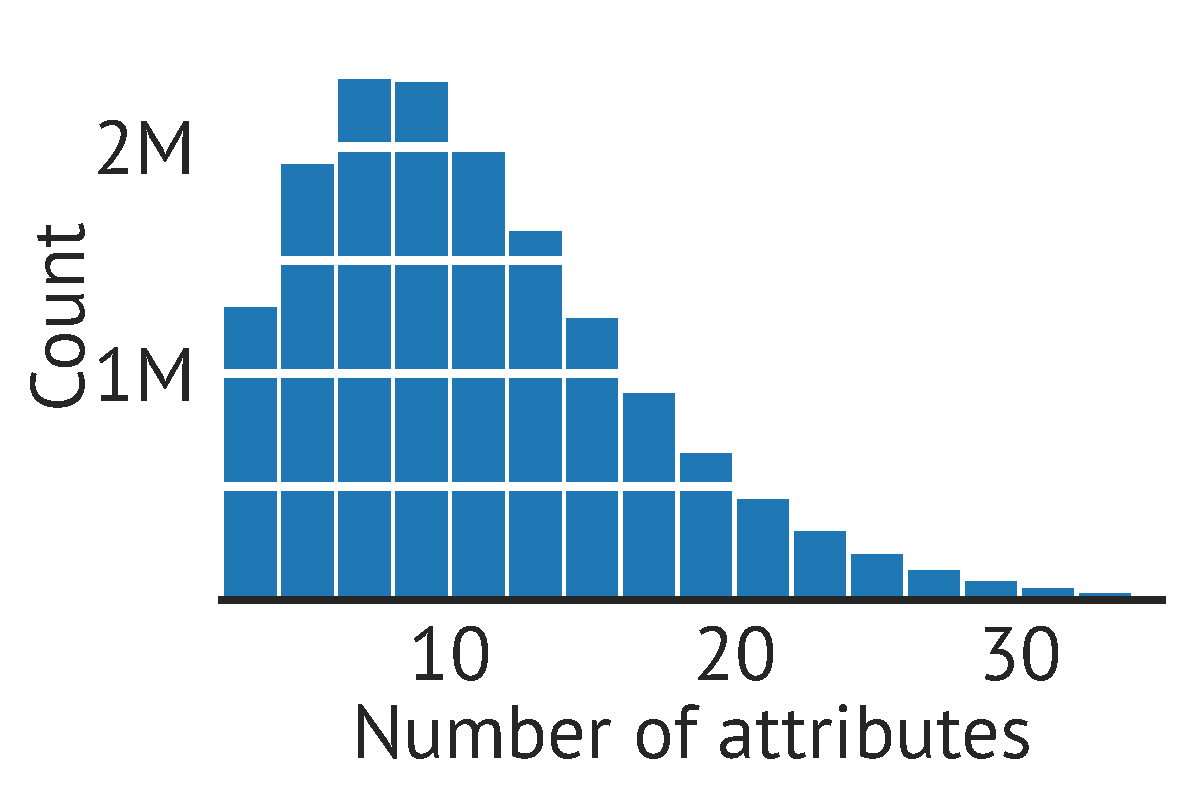
\includegraphics[width=0.6\linewidth]{ch-rfs/fig/hist_meals}
%  \vspace*{-8mm}
  \caption{A histogram of the number of foods illustrates the statistical
    challenge of building models to rank from sets. Even in this subset of the
    data, 50k users consume 16M meals in one year. This means when building a
    model to rank meals, a model with unique parameters for every datapoint is
    inefficient: models should share parameters across meals.}
  % \end{minipage}
  % \begin{minipage}[c]{0.49\linewidth}
  %   \centering
  %   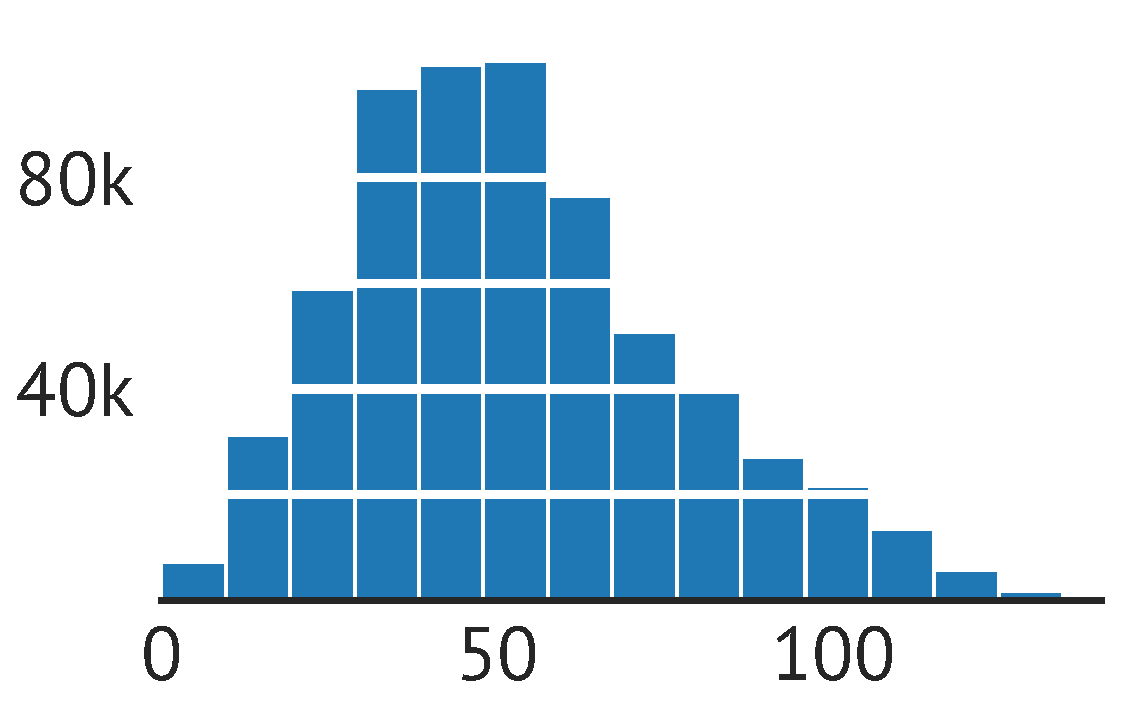
\includegraphics[width=\textwidth]{ch-rfs/fig/hist_arxiv}
  %   \vspace*{-8mm}
  %   \caption*{\# words in arXiv abstracts}
  % \end{minipage}
  % \caption{\textbf{Corpora where items have set-valued attributes have a large
  %     number of unique features.}}
  \label{fig:hist}
\end{figure}

% % hook: why you should read on. world-as-it-could-be if you join us on the ride
% We develop \gls{rfs}, a recommendation model that meets the above
% criteria of parameter-sharing and order-invariance, and guarantees improvement
% in recall and ability to approximate other models. Other order-invariant models
% such as matrix factorization do not have such theoretical backing of improved
% evaluation metrics and ability to approximate other models. The theory we
% develop for \gls{rfs} frees practitioners to focus on building
% efficient architectures for one model, rather than comparing across that may not
% be able to approximate others, or that may not provably improve recall.
% % at a high level, what are the insights needed to solve the problem?
% The key insight that guarantees that \gls{rfs} improves recall is
% the framing of recall as classification. Recall measures the fraction of items a
% user consumed in a ranking returned by a recommendation model. This is
% inherently a binary task: a model does or does not recall an item. It follows
% that a perfect classifier maximizes recall. This framing enables us build
% \gls{rfs} as a classifier and leverage recent innovations from
% deep learning~\citep{Mikolov2013} to fit our model. We define negative samples as
% items users are unlikely to consume. This allows us to fit
% \gls{rfs} to implicit feedback data, where there are only
% user-item interactions, and users do not explicitly indicate dislike of items.
% % universal approximation
% The second goal of building a model that approximates others is achieved by
% parameterizing \gls{rfs} using neural networks. This enables us to
% show that the model can approximate other recommenders that rank from sets. We
% describe several neural network architectures, including one based on residual
% networks~\citep{DBLP:journals/corr/HeZRS15}.
% % describe our model, how it is trained, an how it recommends
% \gls{rfs} is a classifier whose output is the probability of a
% user consuming an item. The model is trained to discriminate items users consume
% from items users are unlikely to consume (negative samples). The probability
% of item consumption output by the model is used to rank items for
% recommendation.
% % deep learning-> universal approximation, and architectures to satisfy
% % order-invariance and parameter-sharing
% We parameterize \gls{rfs} using neural networks, enabling the
% approximation of other models. The architectures of the neural networks are
% defined to meet the criteria of parameter-sharing and order-invariance arising
% from the properties of items represented by sets of attributes.
% % results
% We demonstrate our method by comparing it to several recommendation models on
% two datasets. The first dataset consists of users consuming $16$M meals from a
% food tracking app, and the second consists of users consuming $637$k preprints
% on the arXiv. The model outperforms order-invariant recurrent neural
% networks~\citep{Hochreiter1997}, a word embedding model~\citep{Mikolov2013}, and
% content-based Poisson factorization~\citep{Gopalana}. We also find that
% \gls{rfs} yields interpretable patterns in user behavior as in
% \Cref{fig:arxiv_tsne}.
% \paragraph{Related work.} Regression models such as deep
% sets~\citep{DBLP:journals/corr/ZaheerKRPSS17} have been developed for set-valued
% data. The deep sets model is a regression, not recommendation model, and does
% not use negative sampling in contrast to \gls{rfs}. Several
% recommendation algorithms use negative sampling to improve performance
% \citep{he2017neural,Chen:2017:SSN:3097983.3098202}. There are also deep learning
% models for collaborative filtering~\citep{zhang2017deep}. However, such work is
% centered on recommending items without side information. We focus on items with
% side information comprised of sets of attributes. In this regime the large
% number of unique sets of attributes is an obstacle and requires additional
% modeling choices. \citet{tansey2016diet2vec} also analyze diet data, but do not
% address recommendation. Probabilistic deep learning approaches for
% recommendation exist~\citep{Ranganath:2015} but do not include negative samples
% in the likelihood; we show this improves performance.
% % set up the task of recommendation, foreshadow how we will solve it via
% % classification
% Sets of attributes represent many types of items. A user might be associated
% with a photo that has tags, a disease with diagnosis codes, or a playlist of
% songs. Recommendation models for such items use the item attributes to rank
% items for users. Central to building recommendation models is evaluation, and a
% common metric is recall. But existing models such as matrix factorization do not
% have associated theoretical guarantees of improved recall. Currently, models are
% built on a case-by-case basis and adapted to the data at hand, and must be
% painstakingly compared to see which extension leads to improvement of the
% evaluation metric.
% % foreshadow desiderata
% Our goal is to build a recommendation model to rank items from attributes, and
% buttress the model with theoretical guarantees of universal approximation
% (ability to approximate other models) and of improved recommendation performance
% vis-\`a-vis recall.
% % desideratum #1: statistical challenge
% Building models that rank items from sets of attributes must address two
% difficulties arising from the properties of sets. The first difficulty is the
% statistical challenge posed by the large number of possible sets. The number of
% sets of attributes is large; we cannot posit a model with unique parameters for
% every set of attributes. The meal recommendation problem illustrates this
% statistical challenge. \Cref{fig:hist} shows the number of meals in data from a
% food tracking app. Even in this small fraction of the data, there are over ten
% million unique meals. In building a recommendation model to rank meals based on
% their constituent foods, the model should satisfy the criterion of
% parameter-sharing, and share parameters across meals with similar foods. For
% example, matrix factorization does not satisfy this criteria: it requires
% learning parameters for every meal. This is inefficient, as most meals are
% consumed by a single user in this data. The criterion of parameter-sharing is
% necessary for models to scale to large real-world datasets as in
% \Cref{fig:hist}.
% % desideratum #2
% In addition to parameter-sharing across sets, models that rank items based on
% their sets of attributes must be invariant to the order of set elements. This
% criterion is called order-invariance. For example, a meal is a set of foods, and
% remains the same meal if we permute the foods it contains. Recommendation models
% should yield the same output regardless of the order that set elements are fed
% to the model. Matrix factorization is an example of an order-invariant model.
% \begin{figure}[t!]
  \centering
  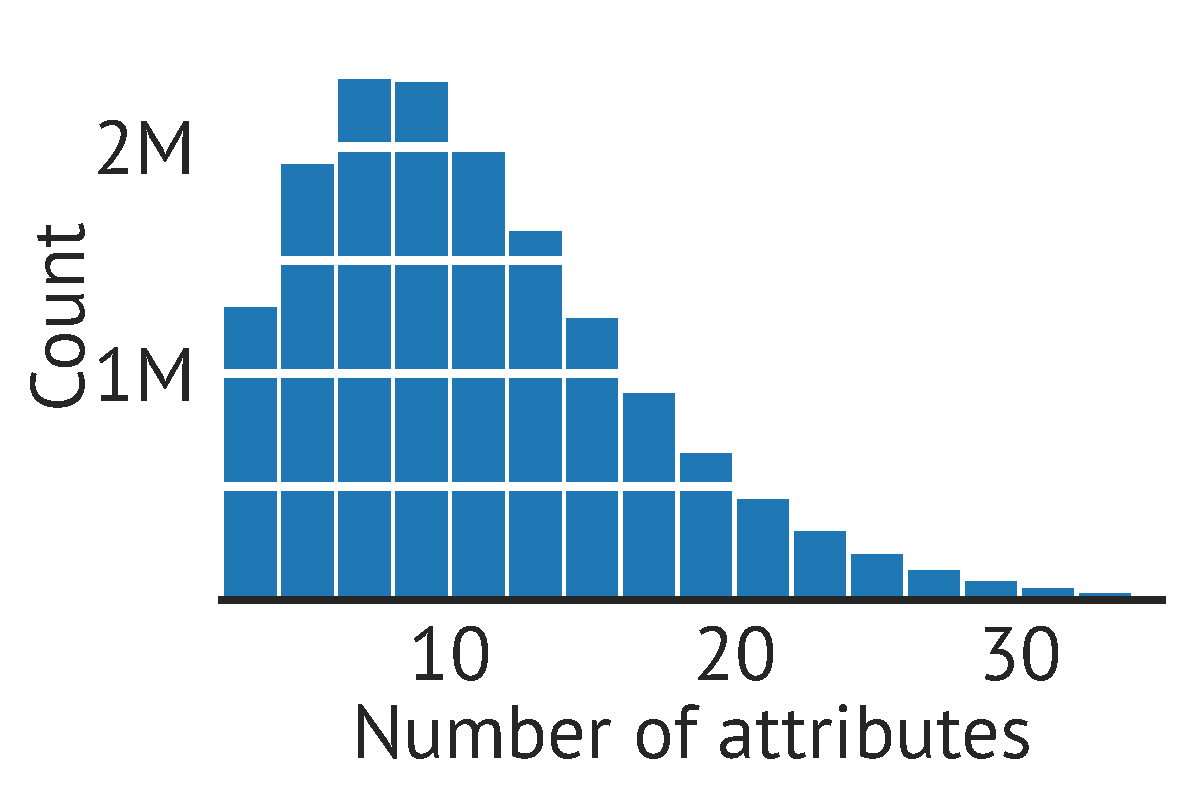
\includegraphics[width=0.6\linewidth]{ch-rfs/fig/hist_meals}
%  \vspace*{-8mm}
  \caption{A histogram of the number of foods illustrates the statistical
    challenge of building models to rank from sets. Even in this subset of the
    data, 50k users consume 16M meals in one year. This means when building a
    model to rank meals, a model with unique parameters for every datapoint is
    inefficient: models should share parameters across meals.}
  % \end{minipage}
  % \begin{minipage}[c]{0.49\linewidth}
  %   \centering
  %   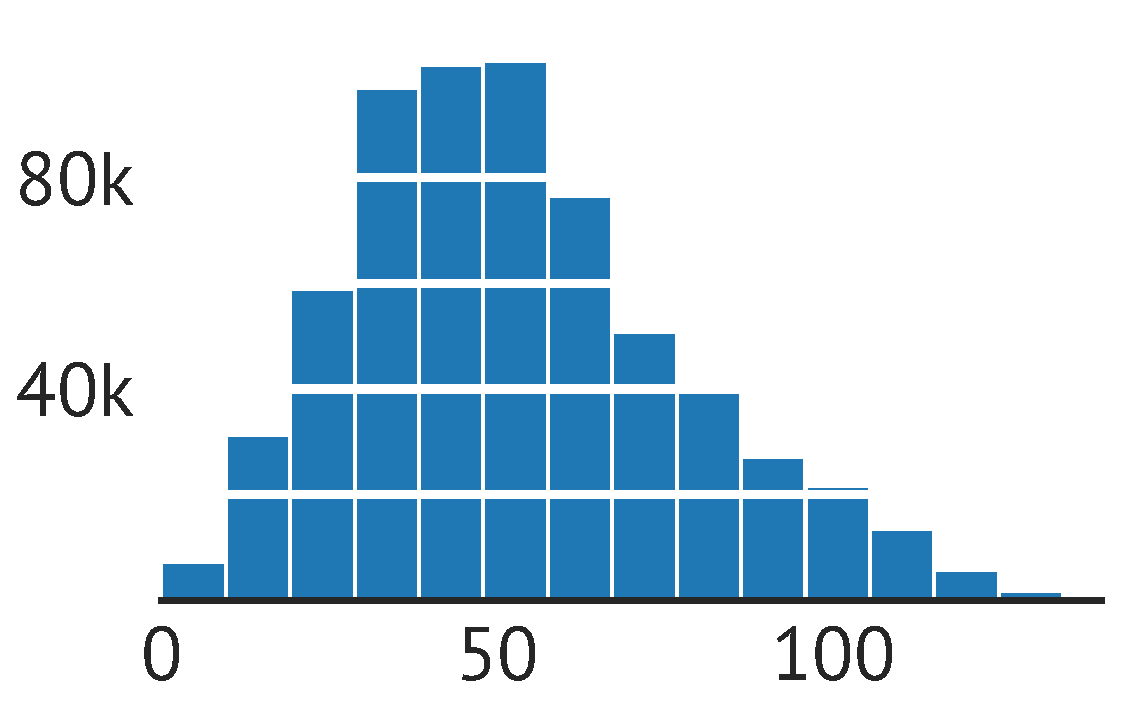
\includegraphics[width=\textwidth]{ch-rfs/fig/hist_arxiv}
  %   \vspace*{-8mm}
  %   \caption*{\# words in arXiv abstracts}
  % \end{minipage}
  % \caption{\textbf{Corpora where items have set-valued attributes have a large
  %     number of unique features.}}
  \label{fig:hist}
\end{figure}

% % hook: why you should read on. world-as-it-could-be if you join us on the ride
% We develop \gls{rfs}, a recommendation model that meets the above
% criteria of parameter-sharing and order-invariance, and guarantees improvement
% in recall and ability to approximate other models. Other order-invariant models
% such as matrix factorization do not have such theoretical backing of improved
% evaluation metrics and ability to approximate other models. The theory we
% develop for \gls{rfs} frees practitioners to focus on building
% efficient architectures for one model, rather than comparing across models that
% may not provably improve recall (or be able to approximate other models).
% % at a high level, what are the insights needed to solve the problem?
% The key insight that guarantees that \gls{rfs} improves recall is
% the framing of recall as classification. Recall measures the fraction of items a
% user consumed in a ranking returned by a recommendation model. This is
% inherently a binary task: a model does or does not recall an item. It follows
% that a perfect classifier maximizes recall. This framing enables us build
% \gls{rfs} as a classifier and leverage recent innovations from
% deep learning~\citep{Mikolov2013} to fit our model. We define negative samples as
% items users are unlikely to consume. This allows us to fit
% \gls{rfs} to implicit feedback data, where there are only
% user-item interactions, and users do not explicitly indicate dislike of items.
% % universal approximation
% The second goal of building a model that approximates others is achieved by
% parameterizing \gls{rfs} using neural networks. This enables us to
% show that the model can approximate other recommenders that rank from sets. We
% describe several neural network architectures, including one based on residual
% networks~\citep{DBLP:journals/corr/HeZRS15}.
% % describe our model, how it is trained, an how it recommends
% \gls{rfs} is a classifier whose output is the probability of a
% user consuming an item. The model is trained to discriminate items users consume
% from items users are unlikely to consume (negative samples). The probability
% of item consumption output by the model is used to rank items for
% recommendation.
% % deep learning-> universal approximation, and architectures to satisfy
% % order-invariance and parameter-sharing
% We parameterize \gls{rfs} using neural networks, enabling the
% approximation of other models. The architectures of the neural networks are
% defined to meet the criteria of parameter-sharing and order-invariance arising
% from the properties of items represented by sets of attributes.
% % results
% We demonstrate our method by comparing it to several recommendation models on
% two datasets. The first dataset consists of users consuming $16$M meals from a
% food tracking app, and the second consists of users consuming $637$k preprints
% on the arXiv. The model outperforms order-invariant recurrent neural
% networks~\citep{Hochreiter1997}, a word embedding model~\citep{Mikolov2013}, and
% content-based Poisson factorization~\citep{Gopalana}. We also find that
% \gls{rfs} yields interpretable patterns in user behavior as in
% \Cref{fig:arxiv_tsne}.
% \paragraph{Related work.} Regression models such as deep
% sets~\citep{DBLP:journals/corr/ZaheerKRPSS17} have been developed for set-valued
% data. The deep sets model is a regression, not recommendation model, and does
% not use negative sampling in contrast to \gls{rfs}. Several
% recommendation algorithms use negative sampling to improve performance
% \citep{he2017neural,Chen:2017:SSN:3097983.3098202}. There are also deep learning
% models for collaborative filtering~\citep{zhang2017deep}. However, such work is
% centered on recommending items without side information. We focus on items with
% side information comprised of sets of attributes. In this regime the large
% number of unique sets of attributes is an obstacle and requires additional
% modeling choices. \citet{tansey2016diet2vec} also analyze diet data, but do not
% address recommendation. Probabilistic deep learning approaches for
% recommendation exist~\citep{Ranganath:2015} but do not include negative samples
% in the likelihood; we show this improves performance.